\documentclass{article}
\usepackage[margin=1in]{geometry}
\usepackage{amsmath, amssymb, amsthm}
\usepackage{enumitem}

\usepackage{makebox}
\newlength{\mymargin}
\settowidth{\mymargin}{\textbf{Category \emph{N}:}}

% color!
\usepackage[dvipsnames]{xcolor}
% \definecolor{mypink1}{rgb}{0.858, 0.188, 0.478}
% \definecolor{mypink2}{RGB}{219, 48, 122}
% \definecolor{mypink3}{cmyk}{0, 0.7808, 0.4429, 0.1412}
% \definecolor{mygray}{gray}{0.6}

% colored links
\usepackage{hyperref}
\hypersetup{
    colorlinks=true,
    linkcolor=blue,
    filecolor=magenta,      
    urlcolor=magenta,
    }

% Inputting psuedocode
\usepackage{algorithm}
\usepackage[noend]{algpseudocode}
\renewcommand\algorithmicdo{}


% Inputting Python code
\definecolor{textblue}{rgb}{.2,.2,.7}
\definecolor{textred}{rgb}{0.54,0,0}
\definecolor{textgreen}{rgb}{0,0.43,0}
\usepackage{upquote}
\usepackage{listings}
\lstset{
    language=Python, 
    tabsize=4,
    basicstyle={\ttfamily},
    keywordstyle=\color{textblue},
    commentstyle=\color{textgreen},
    stringstyle=\color{textred},
    frame=none,
    columns=fullflexible,
    keepspaces=true,
    showstringspaces=false,
    xleftmargin=-15mm, % manual adjustment, figure out permanent solution
}

% tcolorbox
\usepackage{tcolorbox}
\tcbuselibrary{skins,hooks}
\usepackage{varwidth}
\newtcolorbox{mybox}[2][]{enhanced,
    before skip=2mm,after skip=2mm,
    colback=black!5,colframe=black!50,boxrule=0.2mm,
    attach boxed title to top left={xshift=1cm,yshift*=1mm-\tcboxedtitleheight},
    varwidth boxed title*=-3cm,
    boxed title style={frame code={
        \path[fill=tcbcolback!50!black]
        ([yshift=-1mm,xshift=-1mm]frame.north west)
        arc[start angle=0,end angle=180,radius=1mm]
        ([yshift=-1mm,xshift=1mm]frame.north east)
        arc[start angle=180,end angle=0,radius=1mm];
        \path[left color=tcbcolback!80!black,right color=tcbcolback!80!black,
        middle color=tcbcolback!100!black]
        ([xshift=-2mm]frame.north west) -- ([xshift=2mm]frame.north east)
        [rounded corners=1mm]-- ([xshift=1mm,yshift=-1mm]frame.north east)
        -- (frame.south east) -- (frame.south west)
        -- ([xshift=-1mm,yshift=-1mm]frame.north west)
        [sharp corners]-- cycle;
    },interior engine=empty,
    },
fonttitle=\bfseries,
title={#2},#1}


%Images
\usepackage{graphicx}
\usepackage{subcaption}
\usepackage{float}
\newcommand{\glass}{
\includegraphics[height=4ex]{images/glass.png}}
\newcommand{\rum}{
\includegraphics[height=4ex]{images/rum.png}}
\newcommand{\mixedrum}{
\includegraphics[height=4ex]{images/mixed_rum.png}}
\newcommand{\pineapple}{
\includegraphics[height=4ex]{images/pineapple.png}}
\newcommand{\pinacolada}{
\includegraphics[height=4ex]{images/pina_colada.png}}
\newcommand{\mixedpineapple}{
\includegraphics[height=4ex]{images/mixed_pineapple.png}}
\newcommand{\coconut}{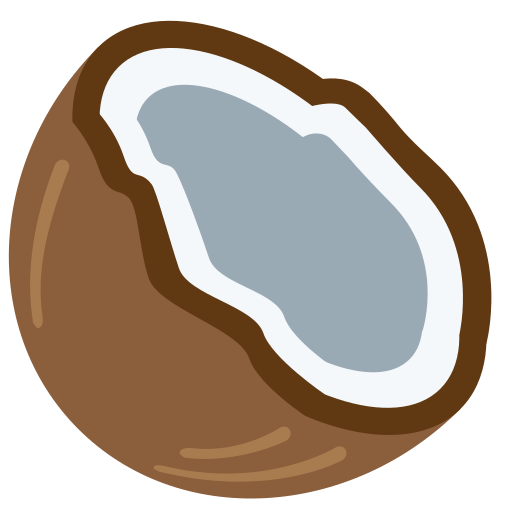
\includegraphics[height=4ex]{images/coconut.png}}
\newcommand{\juice}{\includegraphics[height=4ex]{images/juice.png}}
\newcommand{\heart}{
\includegraphics[height=4ex]{images/heart.png}}
    
%Formatting and Spacing
\setitemize[1]{noitemsep, parsep = 5pt, topsep = 5pt}
\setenumerate[1]{label = (\alph*), parsep = 1pt, topsep = 5pt}
\setlength\parindent{0pt}
\linespread{1.1}

% title
\title{\vspace{-1cm}CS 2051: Honors Discrete Mathematics \\Spring 2023 Homework 7 Supplement}
\author{Sarthak Mohanty}
\date{}

\begin{document}

\maketitle

\section*{Overview}

In recent weeks, we have delved into number theory and explored its practical application in RSA cryptography. However, there is another formidable cryptosystem called Elliptic Curve Cryptography (ECC) that is widely used today to secure various aspects of online communication, ranging from HTTPS connections to inter-data center transmissions. ECC is considered more robust than early public key cryptography systems like RSA, based on current mathematical knowledge. In this supplement, you will learn the algorithmic and mathematical background to understand this cryptosystem, following which you will implement a rudimentary version yourself!\footnote{A good resource for the implementation of this supplement is \cite{ec_blog}.}

\section*{Cryptography Primer}
    In this section, we discuss the difference between symmetric and asymmetric encryption, as well as what constitutes a ``hard" problem in cryptography.

\subsection*{Symmetric vs Asymmetric Systems}

    In cryptography, there are two main types of encryption algorithms: symmetric and asymmetric. 

    \vspace{3mm}
    \textbf{Symmetric}, or \textbf{private-key} encryption uses the same key to both encrypt and decrypt the message. Symmetric encryption algorithms are generally faster and more efficient, but they require the sender and the recipient to share a secret key. The most prominent example is the AES cipher.\footnote{Some of your classmates have chosen this as their group project!} 

    \vspace{3mm}
    On the other hand, \textbf{asymmetric}, or \textbf{public-key encryption} algorithms are slower and less efficient, but they allow the sender to send a message securely to the recipient without sharing a secret key. Examples include RSA, Diffie-Hellman, and ECDH.

\subsection*{Trapdoor Functions}
    
    Trapdoor functions are an essential component of asymmetric encryption algorithms. A trapdoor function is a function that is easy to compute in one direction, but difficult to compute in the opposite direction without knowledge of additional information, such as a secret key.
    
    \vspace{2mm}
    As an example, the trapdoor function in RSA encryption is the \textit{integer factorization problem}: $$\text{Let $N = pq$ be a product of 2 primes with $\log(p) \approx \log(q)$. Given $N$, extract $p, q$.}$$ This is a difficult problem to solve, especially for large values of $p$ and $q$. However, if one has knowledge of the factors $p$ and $q$, computing the value of $N$ is straightforward. This property makes the integer factorization problem an excellent candidate for a trapdoor function.

\section*{Part 1: Diffie-Hellman (10 pts)}
    Before we begin, consider the following story:
    
    \begin{tcolorbox}[colback = CarnationPink!20]
        Professor Brito and Lianet (Brito’s wife!) have a famous Piña Colada recipe that they keep secret from the rest of the world. It is so secret in fact, that neither Brito nor Lianet know the full parts of the recipe! However, using their knowledge on how the Diffie-Hellman key exchange algorithm works, they have devised a unique way of making the drink.
    
        \vspace{2mm}
        To make their famous Piña Colada, Brito and Lianet have their own secret ingredients, which they mix separately. Brito mixes a secret amount of rum to a glass, while Lianet mixes a secret amount of pineapple juice to another glass. These individual mixtures represent the private keys of each party:
        $$\text{Brito:} \glass + \coconut + \rum = \mixedrum \qquad \text{Lianet:} \glass + \coconut + \pineapple = \mixedpineapple$$
        
        \vspace{2mm}
        Next, they swap glasses. This represents the public key exchange. Note that because the ingredients were mixed in, it is very difficult for either Brito or Lianet to determine the exact contents of the current glass.
        $$\text{Brito: \mixedpineapple \qquad Lianet: \mixedrum}$$
        
        Once they have exchanged their mixtures (or ``public keys"), they again use their own secret ingredients (or ``private keys") to mix with the others' drink to generate a shared ``secret key", in this case the final drink.
        $$\text{Brito:} \mixedpineapple + \rum = \pinacolada \qquad \text{Lianet:} \mixedrum + \pineapple = \pinacolada$$
    
        \vspace{2mm}
         This shared secret key can be used to establish a secure communication channel, just like the delicious piña colada they created together.
    \end{tcolorbox}
    Let's now describe any algorithm that can transmit any information, not just piña coladas. 
    
    
\subsection*{Diffie-Hellman Key Exchange}
    The Diffie-Hellman (DH) key exchange is a cryptographic protocol that allows two parties to generate a shared secret key over an insecure communication channel. The protocol is named after its inventors, Whitfield Diffie and Martin Hellman, and is performed as follows:
    \begin{enumerate}[label = \arabic*.]
        \item Alice and Bob agree to use a prime $p$ and a primitive root $g$ of $p$.
        \item Alice chooses a secret positive integer $a < p$ and computes her public key, given by $g^{a} \pmod{p}$. Bob also chooses a secret positive integer $b < p$ and computes his private key, given by $g^{b} \pmod{p}$.
        \item Alice and Bob exchange their respective public keys over an (possibly) insecure channel.
        \item Alice calculates $S = (g^{b} \pmod{p})^{a}$ (using her private key and Bob's public key) and Bob calculates $S = (g^{a} \pmod{p})^{b}$ (using his private key and Alice's public key). Note that they have now computed a shared secret, as $$S = (g^{a} \pmod{p})^{b} = g^{ab} \pmod{p}.$$
    \end{enumerate}

\subsection*{Trapdoor Function: Discrete Log Problem}
    The security of DH comes from the fact that an attacker, even given $g$, $p$, $g^{a} \pmod{p}$, and $g^{b} \pmod{p}$, \underline{cannot} efficiently calculate $g^{ab} \pmod{p}$. This leads us to a trapdoor function known as the \textit{discrete log problem}: $$\text{Given $g$, $p$, and $g^{x}\ \text{mod}\ p$, determine $x$}.$$ We will first demonstrate that we can break the discrete log problem if the parameters $x$ and $p$ are too small. Then, we will see through our implementations that as we increase the size of our numbers, the power of our attacks gets weaker.

    \begin{center}
        \textbf{Brute Force}
    \end{center}

    Recall that we want to find $a$ given $g$, $p$, and $g^{x}\ \text{mod}\ p$. The initial approach one might have would be to try all possible values of $x$. This takes $\mathcal{O}(p)$ time, which follows from the fact that $g$ is a \href{https://en.wikipedia.org/wiki/Primitive_root_modulo_n}{generator}.
    
    \begin{center}
        \textbf{Baby-Step Giant-Step algorithm}
        \footnote{Adapted from \cite{ec_blog}.}
    \end{center}

    Before we describe the algorithm, first note that any integer $x$ can be written as $x = am + b$, where $a$, $m$, and $b$ are arbitrary integers. For example, we can write $10 = 2 \cdot 3 + 4$. With this knowledge, we can rewrite the equation for the discrete log problem as follows:
    \begin{align*}
        g^{x} &\equiv y \pmod{p} \\
        g^{am + b} &\equiv y\pmod{p} \\
        g^{b} &\equiv y \cdot g^{-am} \pmod{p}
     \end{align*}

     The baby-step giant-step is a "meet in the middle" algorithm. In essence, instead of computing $g^{x} \pmod{p}$ for all values $x$, we instead calculate a few values for $g^{b} \pmod{p}$, as well as calculate a few values for $g^{-am} \pmod{p}$. The algorithm works as follows:

     \begin{algorithm}
        \caption{\textsc{BabyStepGiantStep}}
        \label{alg:bsgs}
        \begin{algorithmic}
            \State $m = \lceil \sqrt{p}\ \rceil$
            \For{each $b$ in $0, \dots, m$}
                \State Store $g^{b} \pmod{p}$ in a certain data structure (which one?)
            \EndFor
            \For{each $a$ in $0, \dots, m$}
                \State Check to see if there exists some $g^{b}$ such that $y \cdot g^{-am} \equiv g^{b} \pmod{p}$ (in $\mathcal{O}(1)$ time!)
            \EndFor
            \State \Return $x = am + b$
        \end{algorithmic}
    \end{algorithm}
    To understand why this algorithm works, forget the modulo for a second and take the equation $y = g^{am + b}$. Consider what follows:
    \begin{itemize}
        \item When $a = 0$ we are checking whether $y$ is equal to $g^{b}$, where $b$ is one of the integers from $0$ to $m$.
        \item When $a = 1$ we are checking whether $y$ is equal to $g^{m + b}$. We are comparing $y$ against all exponents from $m$ to $2m$.
        \item When $a = 2$ we are comparing $y$ against all exponents from $2m$ to $3m$.
        \item[\vdots]
        \item When $a = m - 1$, we are comparing $y$ against all exponents from $(m - 1)m$ to $m^{2} = p$.
    \end{itemize}

    In other words, \textbf{we are checking all exponents from $0$ to $p$}. The time complexity of this algorithm is $\mathcal{O}(\sqrt{p})$.

    \pagebreak
    
    \begin{center}
    \textbf{General Number Field Sieve (GNFS)}\footnote{Adapted from \cite{cloudflare_blog}.}
    \end{center}
    
    The General Number Field Sieve is a factorization algorithm that is particularly efficient for numbers with large prime factors. It is a multi-step process that involves finding a smooth polynomial and calculating its roots. GNFS is one of the most efficient known factorization algorithms for large integers.
    
    \vspace{3mm}
    We mention this attack not because of the implementation, but rather due to the implication. Algorithms such as GNFS get more efficient as the size of the numbers being factored get larger. As the resources available to decrypt numbers increase, the size of the keys need to grow even faster. This is not a sustainable situation for mobile and low-powered devices that have limited computational power. For this reason (and others), we need a better public key system. 

    \begin{tcolorbox}[enhanced,interior style={top color=Plum!20,bottom color=Plum!30}]
        In this part, you'll first implement the \lstinline{Actor} class, which contains methods to emulate the Diffie-Hellman key exchange:
    
        \begin{mybox}[
            colframe=Cerulean!50!black,
            colback=Cerulean!30,
            colbacktitle=Cerulean!,
            % fonttitle=\bfseries,
            coltitle=Cerulean!30!black
            ]{Actor}
            A given actor has access to the public parameters $p$ and $g$, as well as its own private key $k$.
            \begin{itemize}
                \item \lstinline{computePublicKey(self)}: Computes and returns the public key.
                \item \lstinline{computeSecret(self, offer)}: Takes in a public key and assigns to the actor the corresponding shared secret.
            \end{itemize}
    
        \end{mybox}
    
        You'll then try to break this key exchange by implementing the \lstinline{BadActor} class, containing the following methods:
    
        \begin{mybox}[
            colframe=purple!50!black,
            colback=purple!30,
            colbacktitle=purple!50!white,
            % fonttitle=\bfseries,
            coltitle=purple!30!black,
            ]{BadActor}
            The bad actor has access to the same public parameters as above, but \underline{not} the private key.
            \begin{itemize}
                \item \lstinline{brute(self, y)}: This function solves the discrete log problem using brute force.
                \item \lstinline{bsgs(self, y)}: This function solves the discrete log problem using the baby-step giant-step algorithm.
                \item \lstinline{stealSecret(self, actor1, actor2, attack)}: This method will use the attacks outlined above to intercept the Actors' shared secret.
            \end{itemize}
            
        These attacks should be reasonably efficient. For example, with parameters $p = 351416641$, $g = 19$ and $a = 137679007$, the following code took 10-20 seconds to brute-force a solution:
        \begin{lstlisting}[belowskip=-6pt]
            alice = Actor("Alice", p, g, a)
            petty_thief = sol.BadActor("Petty Thief", p, g)
            petty_thief.brute_force(alice.computePublicKey())
        \end{lstlisting}
        On the other hand, the baby-step giant-step algorithm below took less than a millisecond!
        \begin{lstlisting}[belowskip=-10pt]
            crime_boss = BadActor("Crime Boss", p, g)
            crime_boss.bsgs(alice.computePublicKey())
        \end{lstlisting}
        
        \end{mybox}
    
        \vspace{2mm}
        Tip: Calculating $g^{a}$ directly and then finding its remainder when divided by $p$ is impractical and will not work with large numbers. This is because $g^{a}$ will be a huge number for large $g, a$. Instead, you should use an algorithm that employs the binary expansion of the exponent $a$.\footnotemark Luckily, Python provides an inbuilt \lstinline{pow} method that performs this algorithm internally.
    \end{tcolorbox}
    \footnotetext{The details of this algorithm can be found in Section 4.2 of the textbook, under ``Modular Expoonentiation".}



\section*{Part 2: Enter Elliptic Curves (8 pts)}
    In this section, we delve into the mathematics behind elliptic curves. The standard form for an elliptic curve is $$y^{2} = x^{3} + ax + b,$$ where $a$ and $b$ are constants. This is referred to as the Weierstrass equation for an elliptic curve. For reasons that will be discussed later, also include the point $\{\infty\}$ in this function.

\subsection*{The Group Law}
    One important aspect of elliptic curves is that we can start with two points, or even one point on an elliptic curve, and produce another point. To do this, start with two points $P = (x_{1}, y_{1})$, $Q = (x_{2}, y_{2})$ on an elliptic curve $E$. Now draw a line $L$ through $P$ and $Q$. This line will intersect $E$ at a third point $R'$. (such a point always exists, as you'll prove below!) Finally, reflect $R'$ across the $x$-axis to obtain $R$. We define $$P + Q = R.$$ You can see an example of this addition in Figure (\ref{fig:point_addition}).

\begin{figure}[htbp]
    \centering
    
    \begin{subfigure}[t]{.45\textwidth}
        \centering
        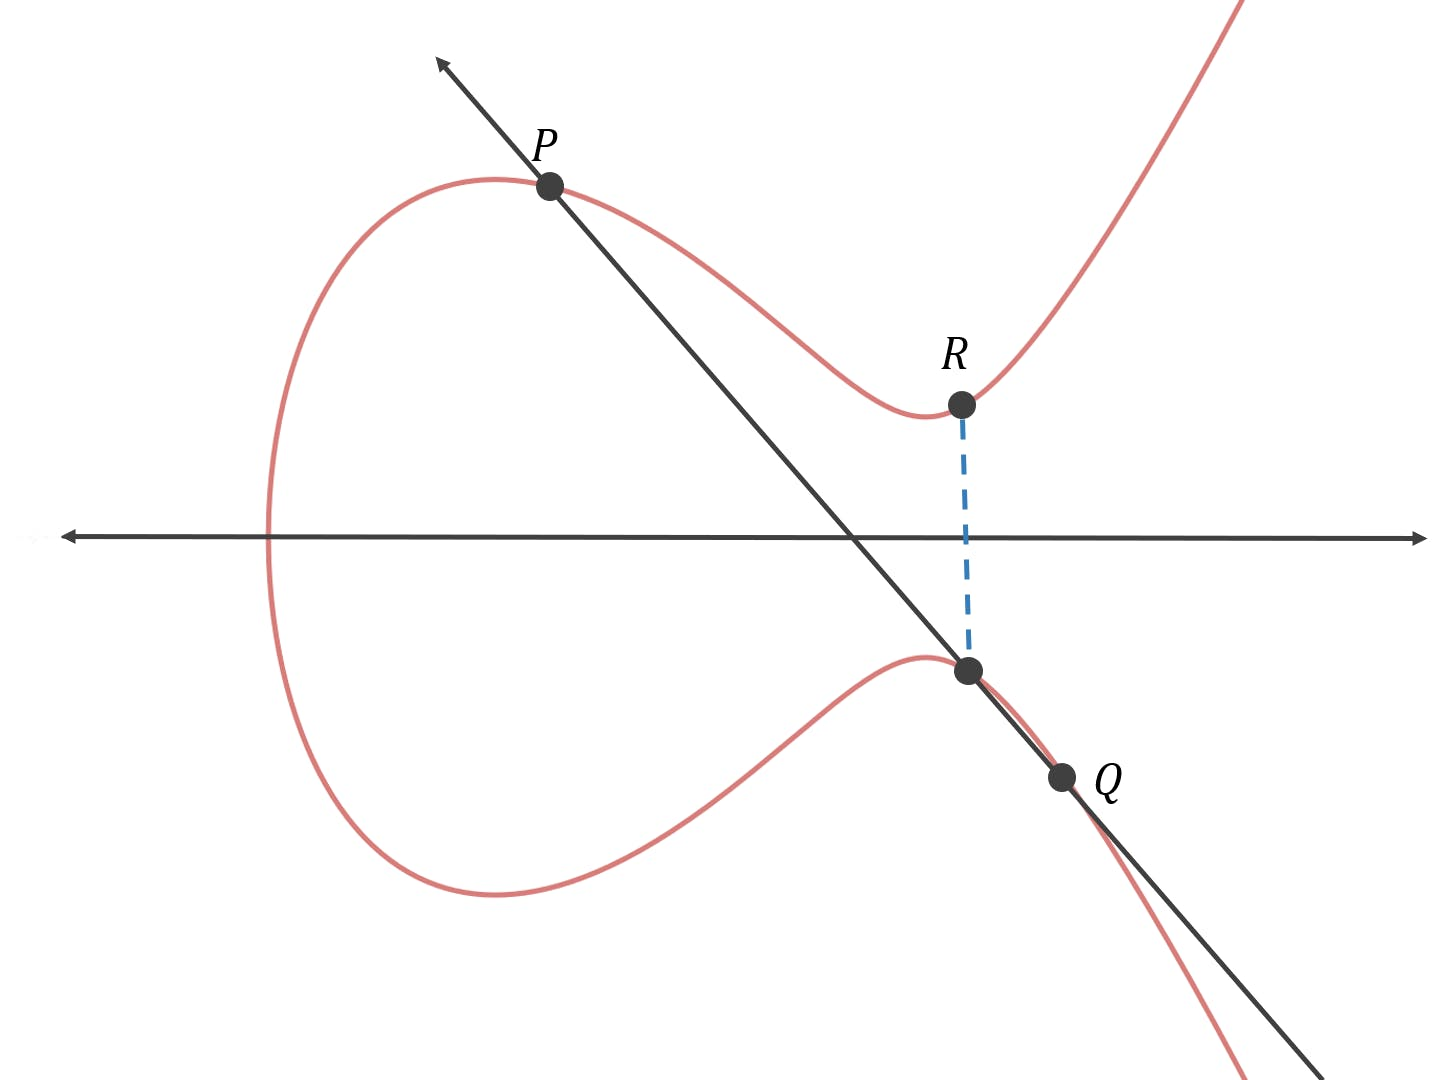
\includegraphics[scale = 0.12]{images/point_addition.jpeg}
        \caption{Point Addition}
        \label{fig:point_addition}
    \end{subfigure}
    \begin{subfigure}[t]{.45\textwidth}
        \centering
        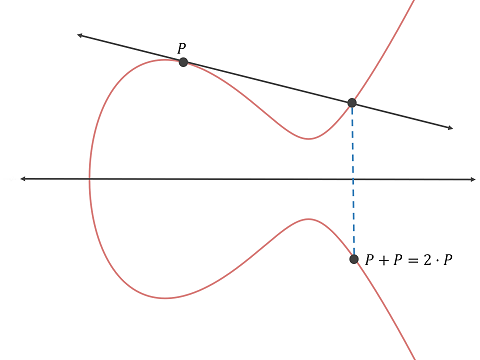
\includegraphics[scale = 0.6]{images/point_scalar_multiplication.png}
        \caption{Point scalar multiplication}
        \label{fig:point_multiplication}
    \end{subfigure}
    \caption{Group law visualized.}
    \label{fig:edge_case}
\end{figure}


\begin{tcolorbox}[enhanced,interior style={top color=Plum!20,bottom color=Plum!30}]
    \textbf{In this part, you'll implement the following functions:}
    \begin{itemize}
        \item \lstinline{point_addition(elliptic_curve, P, Q)}: This function takes in an elliptic curve of the form described as well as two points on the curve $P$ and $Q$, and returns their ``sum".
        \item \lstinline{point_scalar_multiplication(elliptic_curve, k, P))}: This function takes in an elliptic curve of the form described, a scalar integer $k$, and a point $P$, and repeatedly multiplies this result to output a number.
    \end{itemize}
    You can run \lstinline{visualize_addition} and \lstinline{visualize_multiplication} to visualize your points on the curve. I also recommend using this \href{https://andrea.corbellini.name/ecc/interactive/reals-add.html}{interactive webpage} as well (which is honestly much better than mine).

    \vspace{3mm}
    Hint: This part does not require any fanciful coding; just a bit of algebra and calculus. Since I know it's been a while since many of you touched those concepts, here's a few steps you get you started.
    \begin{itemize}
        \item For point addition, assume that $P \ne Q$. For this reason, we can draw the line $L$ through $P_{1}$ and $P_{2}$. Its slope is $$m = \frac{y_{2} - y_{1}}{x_{2} - x_{1}}.$$ If $x_{1} = x_{2}$, then $L$ is vertical, so the resulting point is just $\infty$. Now let's assume that $x_{1} \ne x_{2}$. The equation of $L$ is then $$y = m(x - x_{1}) + y_{1}.$$ To find the intersection of this line with the elliptic curve, we can substitute the above equation into the formula for an elliptic curve $$y^{2} = x^{3} + ax + b.$$ Finally, we can reflect the above point across the $x$-axis to obtain the point $P_{3} = (x_{3}, y_{3})$.
        \item For point scalar multiplication, we have that $P = Q = (x_{1}, y_{1})$. When two points on a curve are very close to each other, the line through them approximates a tangent line. Therefore, when the two points coincide, we take the line $L$ through them to be the tangent tine. Implicit differentiation allows us to find the slope $m$ of $L$: $$2y \frac{dy}{dx} = 3x^{2} + a,\text{\quad so\quad} m = \frac{dy}{dx} = \frac{3x_{1}^{2} + a}{2y_{1}}.$$ If $y_{1} = 0$ then the line is vertical and we set $P_{1} + P_{2} = \infty$, as before. Otherwise, we plug in values into $L$ and solve as before. To make this algorithm efficient, you may want to look up the ``square-and-multiply" method.
    \end{itemize}
    
\end{tcolorbox}

\section*{Part 3: In The Field (12 pts)}
    The simplified curve above is great for visualization and to explain the general concept, but it doesn't really represent how the curves used for cryptography look like. Just like in RSA, we have to restrict ourselves to a fixed range of numbers.

    \vspace{3mm}
    The elliptic curve cryptography (ECC) uses elliptic curves taken over the finite field $\mathbb{F}_{p}$, where $p$ is a prime number. For example, the ``Bitcoin curve" secp256k1 takes the form: $$y^{2} \equiv x^{3} + 7 \pmod{p}.$$ Figure 2 shows an illustration of the curve taken over $\mathbb{R}$ and $\mathbb{F}_{97}$.

    \vspace{2mm}
    ECC only works with curves under such fields, so we need to modify our group law to support these. Luckily, the group law is near-identical (with a few changes, both of which are explained in \cite{ec_blog})

    \begin{figure}[htbp]
        \centering
        
        \begin{subfigure}[t]{.45\textwidth}
            \centering
            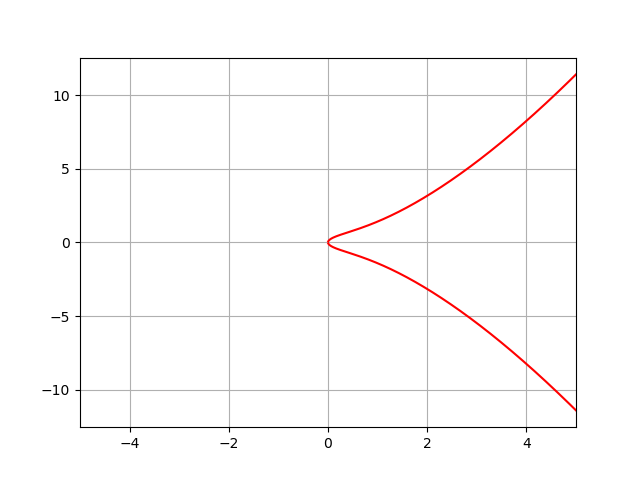
\includegraphics[scale = 0.4]{images/curve.png}
            \caption{The bitcoin curve over $\mathbb{R}$}
            \label{fig:point_addition}
        \end{subfigure}
        \begin{subfigure}[t]{.45\textwidth}
            \centering
            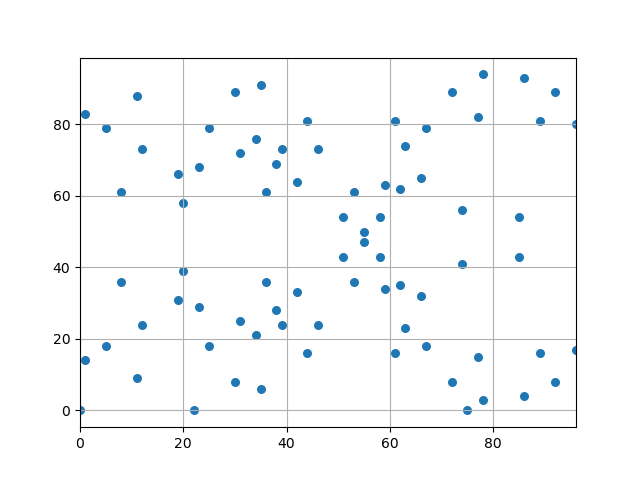
\includegraphics[scale = 0.4]{images/curve_over_field.png}
            \caption{The bitcoin curve over $\mathbb{F}_{97}$.}
            \label{fig:point_multiplication}
        \end{subfigure}
        \caption{Visualizing elliptic curves over a field.}
        \label{fig:edge_case}
    \end{figure}

    \begin{tcolorbox}[enhanced,interior style={top color=Plum!20,bottom color=Plum!30}]
        In this part, you'll visualize elliptic curves over finite fields, as well as implement point addition and point multiplication over these fields
    
        \textbf{In this part, you'll implement the following functions:}
        \begin{itemize}
            \item \lstinline{generate_point_cloud(a, b, p)}: This takes in an elliptic curve and returns the set of all valid points in the curve over that field, including the point at infinity.
            \item \lstinline{point_addition(P, Q, a, b, p)}: This function takes in an elliptic curve (now over a finite field) and two points. It returns their point-wise sum.
            \item \lstinline{point_scalar_multiplication(P, k, a, b, p)}: This function takes in an elliptic curve of the form above, a scalar integer $k$, and a point $P$, and repeatedly multiplies $P$ $k$ times.
        \end{itemize}
        After completing each function, you should be able to run \lstinline{visualize_curve}, \lstinline{visualize_point_addition}, and \lstinline{visualize_point_scalar_multiplication} to check your work, as well as the \href{https://andrea.corbellini.name/ecc/interactive/reals-add.html}{interactive tool} mentioned above.
    \end{tcolorbox}

\section*{Part 4: ECC in Action: Elliptic-curve Diffie Hellman (10 pts)}

\subsection*{The Elliptic-curve Discrete Log Function}
    Finally, the part you've been waiting for. With our newfound knowledge about elliptic curves, we can make the DH key exchange much more powerful, as follows
    \begin{enumerate}[label = \arabic*.]
        \item Alice and Bob agree to use a curve $c = (a, b, n)$ and a generator point $P$.
        \item Alice chooses a secret positive integer $k_{a} < n$ and computes her public key, given by $k_{a}P$. Bob also chooses a secret positive integer $k_{b} < n$ and computes his public key, given by $k_{b}P$.
        \item Alice and Bob exchange their respective public keys over an (possibly) insecure channel.
        \item Alice calculates $S = k_{a}(k_{b}P)$ (using her private key and Bob's public key) and Bob calculates $S = k_{b}(k_{a}P)$ (using his private key and Alice's public key). Note that they have now computed a shared secret, as $$S = k_{a}(k_{b}P) = k_{b}(k_{a}P).\footnote{The proof of this property can be found in \cite{ec_book}}$$
    \end{enumerate}

\subsection*{The Elliptic-curve Discrete Log Function}
    The security of this cryptosystem follows from yet another trapdoor function, let's call it the \textit{elliptic-curve discrete log problem}: $$\text{Given a curve, $Q$, and $P$, determine $k$ such that $Q = kP$}.$$ Once again, this problem has no efficient solution. Note the similarity to the original discrete log problem. The attacks are similar as well, and can be found in $\cite{ec_blog}$

    % Trapdoor function in Elliptic Curve Cryptography (ECC). In ECC, the trapdoor function is the scalar multiplication operation $Q = kP$, where $P$ is a point on the elliptic curve, $k$ is the scalar and $Q$ is the result of the scalar multiplication. The trapdoor information is the private key, which is the scalar $k$. Decryption is performed by computing $Q = -kP$. For carefully chosen (by cryptographers) finite fields and elliptic curves, the ECDLP problem has no efficient solution. The multiplication of elliptic curve points in the group $\mathbb{F}_{p}$ is similar to exponentiation of integers in the group $\mathbb{Z}_{p}$ (this is known as multiplicative notation) and this is how the ECDLP problem is similar to the DLP problem (discrete logarithm problem).


    \begin{tcolorbox}[enhanced,interior style={top color=Plum!20,bottom color=Plum!30}]
        In this part, you'll implement an Elliptic-Curve Diffie Hellman key change algorithm. The functions you will implement are similar to those in Part 1. First, you'll implement the \lstinline{Actor} class:
    
        \begin{mybox}[
            colframe=Cerulean!50!black,
            colback=Cerulean!30,
            colbacktitle=Cerulean!,
            coltitle=Cerulean!30!black
            ]{Actor}
            A given actor has access to the public curve parameters $(a, b, n)$, the public generator point $P$, and a private key $k$.
            \begin{itemize}
                \item \lstinline{computePublicKey(self)}: Computes and returns the public key.
                \item \lstinline{computeSecret(self, offer)}: Takes in a public key and assigns to the actor the corresponding shared secret.
            \end{itemize}
    
        \end{mybox}
    
        Then, the \lstinline{BadActor} class.
    
        \begin{mybox}[
            colframe=purple!50!black,
            colback=purple!30,
            colbacktitle=purple!50!white,
            % fonttitle=\bfseries,
            coltitle=purple!30!black,
            ]{BadActor}
            The bad actor has access to the same public parameters as above, but \underline{not} the private key.
            \begin{itemize}
                \item \lstinline{brute(self, Q)}: This function solves the ECDLP using brute force.
                \item \lstinline{bsgs(self, Q)}: This function solves the ECDLP using the baby-step giant-step algorithm.
                \item \lstinline{stealSecret(self, actor1, actor2, attack)}: This method will use the attacks outlined above to intercept the Actors' shared secret.
            \end{itemize}
        \end{mybox}
        Again, to receive full credit, these attacks should be reasonably efficient. You may also want to double-check the efficiency of your methods developed in Part 3, since they should be used in this section.
    \end{tcolorbox}

\subsection*{Conclusion}

    \subsubsection*{RSA vs ECC}

    Since RSA and ECC essentially serve the same purpose, there have been many heated discussions as to which implementation to use. The main pro of using ECC is the fact that it uses fewer memory and CPU resources, important as mobile computing becomes more ubiquitous. However, there are a few flaws with ECC.
    
    \vspace{2mm}
    Finally, neither ECC nor RSA are secure against quantum computers. Even if quantum computers are not ready to be deployed at scale yet, lots of information is being stored now with intentions of being decrypted later. This has spurred \href{https://csrc.nist.gov/projects/post-quantum-cryptography}{calls} to create quantum-resistant encyption schemes.

    \subsubsection*{Real World Applications}

    Even with all those downsides, more and more companies are using ECC, including

    \begin{center}
        Amazon, Bing, Dropbox, Facebook, Flickr, GitHub, Instagram, \\
        LinkedIn, MSN, Netflix, Pinterest, PirateBay, Quora, Snapchat, \\
        SoundCloud, Spotify, StackOverflow, Tumblr, Twitter, Uber, \\
        Vimeo, Vine, Yahoo, Yelp, YouTube, Wikipedia, Wordpress,\dots
    \end{center}
    Even \href{https://chat.openai.com/chat}{ChatGPT} is using ECC to establish their connections, which you can check yourself. In Chrome, clicking on the lock in the address bar and traversing to the connection tab shows which cryptographic protocols were used in establishing the secure connection. ECC should be listed as one of them.

    \vspace{3mm}
    However, as noted in the beginning of this supplement, symmetric encryption schemes are much faster than their asymmetric counterparts. This is why in practice, most information is transferred using symmetric encryption schemes such as AES. This does not mean asymmetric schemes are useless; in practice, both encryption schemes are usually used in tandem. You can see an example of such ``hybrid" symmetric-asymmetric schemes \href{https://github.com/nakov/Practical-Cryptography-for-Developers-Book/blob/master/asymmetric-key-ciphers/ecc-encryption-decryption.md}{here}.

\section*{Submission Instructions (10 pts)}
    After you fill the appropriate functions, submit the following files to Gradescope and make sure you pass all test cases:
    \begin{itemize}
        \item \lstinline{diffie_hellman.py}
        \item \lstinline{elliptic_curves.py}
        \item \lstinline{ECDH.py}
    \end{itemize}

    \vspace{3mm}
    \textbf{Notes}
    \begin{itemize}
        \item The autograder may not reflect your final grade on the assignment. We reserve the right to run additional tests during grading.
        \item Do not import additional packages, as your submission may not pass the test cases or manual review.
    \end{itemize}

\begin{thebibliography}{9}
    \bibitem{ec_book}
    Washington, L. C. (2008). \textit{Elliptic curves: number theory and cryptography (2nd ed.).} Chapman and Hall/CRC.

    \bibitem{ec_blog}
    Corbellini, A. (2015). \textit{Elliptic Curve Cryptography: a Gentle Introduction.} Retrieved from https://andrea.corbellini.name/2015/05/17/elliptic-curve-cryptography-a-gentle-introduction/
    
    \bibitem{cloudflare_blog}
    Sullivan, N. (2023, October 23). A (Relatively Easy To Understand) Primer on Elliptic Curve Cryptography. The Cloudflare Blog. https://blog.cloudflare.com/a-relatively-easy-to-understand-primer-on-elliptic-curve-cryptography/.
\end{thebibliography}

\end{document}